\begin{figure}[h] 
\centering 
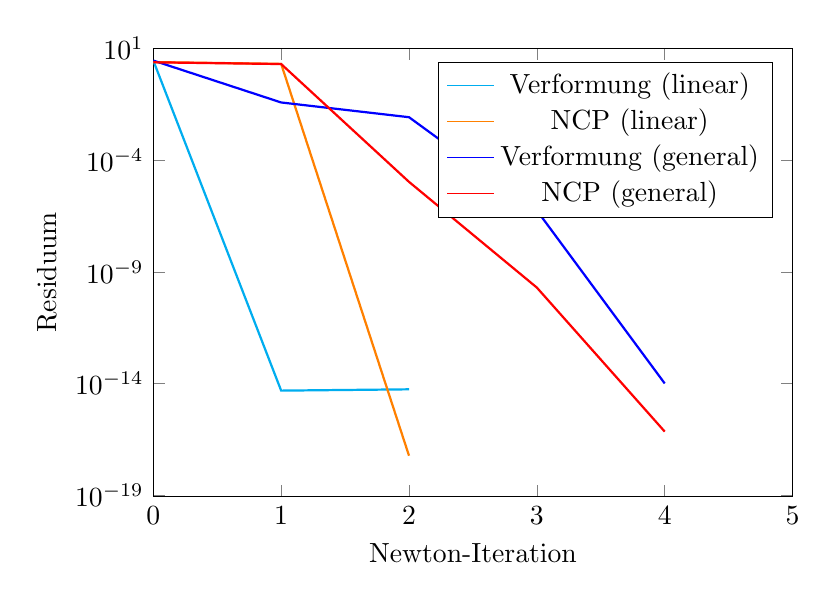
\begin{tikzpicture}[every plot/.append style={thick}] 
\begin{axis}[ 
label style={font=\normalsize}, 
xlabel={Newton-Iteration}, 
ylabel={Residuum}, 
xmin=0, xmax=5, 
ymode=log, 
ymin=0, ymax=10, 
width=0.8\textwidth, 
height=0.6\textwidth, 
legend pos=north east, 
legend style={cells={align=left}}, 
grid style=dashed, 
] 
\addplot[ 
color=cyan, 
] 
coordinates { 
(0, 2.78e+00)(1, 4.87e-15)(2, 5.57e-15)}; 
\addlegendentry{Verformung (linear)} 
\addplot[ 
color=orange, 
] 
coordinates { 
(0, 2.38e+00)(1, 1.98e+00)(2, 5.98e-18)}; 
\addlegendentry{NCP (linear)} 
\addplot[ 
color=blue, 
] 
coordinates { 
(0, 2.79e+00)(1, 3.73e-02)(2, 8.18e-03)(3, 5.54e-07)(4, 1.02e-14)}; 
\addlegendentry{Verformung (general)} 
\addplot[ 
color=red, 
] 
coordinates { 
(0, 2.33e+00)(1, 1.95e+00)(2, 1.05e-05)(3, 1.97e-10)(4, 7.18e-17)}; 
\addlegendentry{NCP (general)} 
\end{axis} 
\end{tikzpicture} 
\caption{Residuen des Stoffgesetzes 'Linear elastisch' mit Hinderniss 'Parabel' und 162 Freiheitsgraden für die Verschiebung.} 
\label{fiq:Linearelastisch_Parabel_level2} 
\end{figure} 
